\documentclass{abrice}

\title{Comp 491: Capstone Proposal}
\author{Anthony Brice\protect\\\medskip David Claveau, PhD.}
\date{\today\protect\\ \bigskip Aggregate Metadata Browsing Over HTTP}

\usepackage[style=nature,natbib=true,backend=biber]{biblatex}
\addbibresource{proposal.bib}

\usepackage{flowchart}
\usetikzlibrary{arrows}

\usepackage{pgfgantt}

\setcounter{secnumdepth}{2}

\begin{document}
\maketitle

\section{Introduction}

Many music players, especially web-based, give the user very little control
over the ways in which one can sort and filter music. Miller columns have come
to be the de facto standard for browsing and visualizing a music database, but
most players only give the user a few columns tied to particular metadata, like
the common Album Artist--Album sort. Those that do allow the user to define an
arbitrary number of columns on arbitrary metadata are exclusively native
applications which expect their database and physical music files to be located
on the same device. This capstone proposes a client--server application with a
centralized music database communicating with many web-based clients allowing a
rich set of sorting and filtering capabilities.

\section{Background}

The problem of digital asset management, especially as it pertains to large
music libraries, is not a new one. Many metadata browsers exist but vary widely
in the control they give to their users over the ability to sort and
filter. Apple's iTunes for example, easily the most ubiquitous media player,
allows the user to sort by year but not filter.

Musicbee, a popular third-party media player that serves as the inspiration for
this proposal, provides the user with up to 6 miller columns with which one can
sort and filter the database~\cite{musicbee}. Unfortunately it is also a
closed-source application native to Windows only.

Quod Libet, an open-source and cross-platform media player, takes the novel
approach of foregoing a traditional database in favor of creating serialized set
of Python objects with which to query~\cite{quodlibet}. This choice may be too
clever for its own good, as filters over as few as three metadata frames tend to
require quite large amounts of RAM for large databases (on the order of 1GB for
60K music files). Like the previous examples Quod Libet is also a native desktop
application that expects its database and files to reside on the same physical
device.

Subsonic is a popular client--server media player and another inspiration for
this proposal~\cite{subsonic}. It offers an easy-to-use web interface connected
to a server but only provides a few canned sorts, such as Album Artist--Album
and randomized Genre playlists.

\section{Requirements}

As shown in Fig.~\ref{fig:arch}, the program will have the common
database/application/client structure. Any source written in service of
implementation will be licensed under version 3 of the GNU General Public
License.

\begin{figure}
  \label{fig:arch}
  \centering
  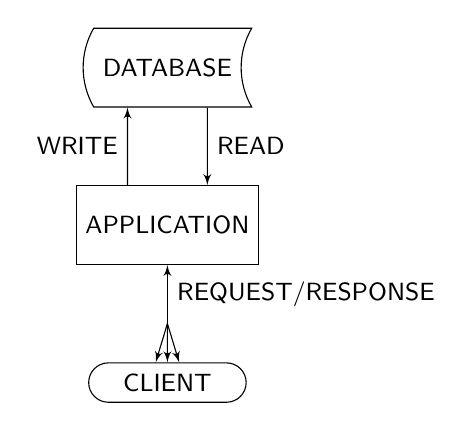
\begin{tikzpicture}[>=latex',font={\sffamily \small}]
    \def\smbwd{2cm}

    \node (database) at (0,0) [draw, storage,
    minimum width=\smbwd,
    minimum height=1cm] {DATABASE};

    \node (application) at (0,-2) [draw, process,
    minimum width=\smbwd,
    minimum height=1cm] {APPLICATION};

    \coordinate (point1) at (0,-3.25);

    \node (client) at (0,-4) [draw, terminal,
    minimum width=\smbwd,
    minimum height=0.5cm] {CLIENT};

    \draw[->] (database.-45) -- node[right]{READ} (application.45);
    \draw[->] (application.135) -- node[left]{WRITE} (database.225);
    \draw[<-] (application) -- node[right]{REQUEST/RESPONSE}(point1);
    \draw[->] (point1) -- (client.120);
    \draw[->] (point1) -- (client.90);
    \draw[->] (point1) -- (client.60);
  \end{tikzpicture}
  \caption{A block diagram describing the proposal's architecture.}
\end{figure}

\subsection{Functional Requirements}

The program will provide a Web interface to an online music database,

% The database will reside on a server and provide a model of the metadata of
% locally stored audio files with which the application layer can interact. The
% database will accept queries and output either a list of values for a particular
% metadata frame or a list of files matching a particular set of metadata
% values. The database will allow the modification of metadata during run-time.

% The application layer will reside on a web-server and provide a means of
% communication between the client and the database. The application layer will
% accept queries from the client, forward them to the database, and send the
% response back processed for transport via HTTP\@. The application layer will
% handle hosting and serving the initial load for the client web application, and
% will provide authentication and authorization for various user roles, such as
% only allowing registered users to play and view the database and only
% administrators to modify the metadata. The application layer will ensure that
% any request to change metadata is written both to the database and the actual
% music files.

% The client will make heavy use of the miller column visualization technique to
% provide an interface through which a user can easily sort and filter the files
% in the database into a playlist which he or she can then play. The client will
% run on any hardware that can run a traditional web browser, with the latest
% version of Mozilla Firefox being the specified target platform. The client will
% respond gracefully to different sized viewports; i.e.\ the client will not
% attempt to detect the device on which the client is being served and serve an
% appropriate front-end, but instead serve a common client that reacts to changes
% in the size of the viewport.

\subsection{Performance Requirements}

The database must have the ability to sort quickly and efficiently an
arbitrarily large number of metadata records. To accommodate any number,
performance should scale linearly as commodity-hardware servers are added to a
cluster.

The application layer should respond to requests with either raw packets over
HTTP (for development) or compressed and minimized packets over HTTPS (for
production). The database and application layers should be capable of handling
100 clients per server of cost outlined below. More and better hardware should
allow this number to scale linearly.

As per common general usability guidelines, a client over a reasonably fast
Internet connection (say, no less than 1 MB-per-second download and upload)
should expect a complete response from the server within 2 seconds.

\subsection{Cost}

Hardware for a server capable of handling at least 100\,000 metadata records
should cost no more than 500~USD\@. Free and open-source software will comprise
the entirety of third-party components such as the database management system.

Any computer capable of running a web browser reasonably well, such as a 50~USD
Raspberry Pi, should be capable of running the web client.

\section{Implementation}

The choice between a traditional SQL or document-oriented database is
non-obvious and will likely be determined through experimentation. A
document-oriented database such as MongoDB or Couchbase is desirable because of
their schema-less nature. I would like to avoid defining specific metadata
frames on which the client can sort since the ID3 specification allows the
creation of arbitrary frames. In addition these databases scale linearly on
commodity hardware, so there's little worry that a database could get too big to
function. Conversely, a document-oriented database may be undesirable because
the client does use the data in a very relational way, and I am unsure if they
can handle the queries I plan to support.

The application layer can be implemented in a number of existing web
frameworks. The nature of database-driven applications requires that the
application be tightly coupled to the database implementation, so it seems
simplest to me to pass that requirement onto the client, since having the
application define its own query language would not loosen the coupling but only
make the client tightly coupled to this application. As I see it, the
application layer should take take queries from the client in the database's
native language, pass them on to the client, and serve up the results. I will
experiment with allowing the application to keep cursors open to allow the
streaming of result sets in an asynchronous way (like how Gchat makes
asynchronous requests for one's chat history as one scrolls a chat window up),
but I do not know well this will scale since in the worst case it requires an
open database connection for every client.

The client will be served in standard HTML5/CSS/ECMAScript. It will be a
single-page application making heavy use of AJAX requests to deliver content.  I
would like to use a new functional-reactive DSL called Elm, which provides a
clean, Haskell-like syntax for defining such applications \cite{czaplicki}. I
believe the modularity inherent to its pure and immutable design and the
performance benefits from its abstract ``virtual DOM'' (i.e.\ scene graph)
implementation will be quite useful to my front-end.

\section{Project Plan}

\begin{figure}
  \centering
  \begin{ganttchart}[
    vgrid,
    title label font={\sffamily \small},
    bar label font={\sffamily \small},
    milestone label font={\sffamily \small \itshape\/}
    ]{1}{15}
    \gantttitle{Spring 2016}{15} \\
    \gantttitlelist{1,...,15}{1} \\
    \ganttbar{Dev. DB}{1}{3} \\
    \ganttlinkedbar{Dev. App. Layer}{2}{9} \\
    \ganttmilestone{Feature Complete}{7} \ganttnewline[]
    \ganttlinkedbar{Dev. Client}{4}{12} \\
    \ganttmilestone{Finalize API}{10} \ganttnewline[]
    \ganttlinkedbar{Presentation Prep.}{13}{15}
    \ganttlink{elem1}{elem2}
    \ganttlink{elem3}{elem4}
  \end{ganttchart}
  \caption{A Gantt chart describing the proposal's schedule.}
\end{figure}

\noindent
I have broken the project into four distinct phases with two milestones
throughout. The phases divide into three development phases---the database,
application, and client components---and a final phase for presentation
preparations.

The database development phase should move quickly as it only entails a few,
relatively simple items: configuring and spinning up a database, writing a
program to handle importing a set of music files into the specific DBMS, and
writing documentation for configuration and the use of the import program.

Next started will be the application phase, and a few weeks into that I should
be ready to begin work on the client as well. Most work on both these layers
will be done in tandem. I expect to require a clear understanding of the
client's needs in order to offer the most useful API from the server-side
application.

By week 7 I plan to have a feature-complete rough draft of my project. This may
seem early, but I expect the application to perform rather poorly at this point
and wish to leave a significant amount of time for tuning. By week 10 I expect
to be ready to finalize the application layer's API, spending weeks 11 and 12
polishing the client GUI\@. I leave 3 weeks at the end of the semester to
prepare for capstone presentations.

\printbibliography%

\end{document}
%%% Local Variables:
%%% mode: latex
%%% TeX-master: t
%%% End:
